\documentclass[conference]{IEEEtran}
\IEEEoverridecommandlockouts
\usepackage{cite}
\usepackage{amsmath,amssymb,amsfonts}
\usepackage{graphicx}
\usepackage{float}
\usepackage{caption}
\usepackage{textcomp}
\usepackage{newunicodechar}
\usepackage{xcolor}
\usepackage{hyperref}
\usepackage{booktabs}

\begin{document}

\title{ARniture: Immersive 3D Furniture Visualization for Modern Living}

\author{
Sneha M. Yadav\thanks{Dept. of Artificial Intelligence and Data Science Vidyavardhini's College of Engineering and Technology, Mumbai, India. Email: sneha.yadav@vcet.edu.in} \and 
Aryan Prakash Koli\thanks{Dept. of Artificial Intelligence and Data Science Vidyavardhini's College of Engineering and Technology, Mumbai, India. Email: aryan.236107102@vcet.edu.in} \and 
Piyush Vitthal Kurwade\thanks{Dept. of Artificial Intelligence and Data Science Vidyavardhini's College of Engineering and Technology, Mumbai, India. Email: piyush.236117106@vcet.edu.in} \and 
Shubham Jagannath Parande\thanks{Dept. of Artificial Intelligence and Data Science Vidyavardhini's College of Engineering and Technology, Mumbai, India. Email: shubham.236237101@vcet.edu.in}
}

\maketitle

\begin{abstract}
In this paper, a complete method of furniture visualization is presented by converting 2D images into interactive 3D objects and presenting them in augmented reality spaces. With Flutter used for cross-platform deployment, ARCore for the feature of augmented reality, and the Meshy AI API to generate 3D models, the system has a smooth, user-friendly interface to visualize furniture products in actual locations. The method combines a product list that has been sorted with Firebase for authentication and database storage, to ensure that after being generated, models are readily stored and easily accessed for later use. Such a system, apart from enabling more extensive online furniture shopping with users being able to view and interact with furniture online in advance also showcases substantial improvements in scalability, efficiency, and user interaction for AR-based retail use.
\end{abstract}

\begin{IEEEkeywords}
furniture visualization, 2d-to-3d conversion, augmented reality, arcore, meshy ai api, firebase integration, flutter framework, 3d model generation, interactive ar experience, user-centric design
\end{IEEEkeywords}

\section{Introduction}
Augmented Reality (AR) has also been a disruptive technology allowing digital content to be linked with physical experience, allowing real-time, interactive user interaction with virtual objects \cite{ref1}. Its use has expanded extensively in retailing, allowing it to make it possible to achieve new customer satisfaction improvement and touchpoints \cite{ref15}, \cite{ref16}. AR is one of the most viable applications of AR to be used in furniture retailing because customers often find it difficult to visualize how a product will be interpreted and redefined in their own domains. This paper proposes an AR-based Furniture Visualization system that transforms 2D images of furniture into interactive 3D models, where users can put and move these models virtually in real-world environments using mobile phones \cite{ref11}, \cite{ref12}. We use a mixture of contemporary software platforms and tools to enable this system. Flutter framework is utilized in developing a dynamic and interactive cross-platform mobile app \cite{ref3}, \cite{ref9}, \cite{ref17}, and Google ARCore SDK enables accurate tracking and rendering of 3D objects into the real world \cite{ref2}, \cite{ref7}. The center of attention in our solution is using Meshy AI API, which directly generates the 2D images of furniture to be automatically translated to 3D models without 3D modeling manually \cite{ref5}. Firebase also handles real-time authentication, secure storage of users' data, and loading of pre-trained models \cite{ref4}, \cite{ref18}, \cite{ref19}. Conventional e-commerce websites heavily depend on static images and descriptions, leading to ambiguity and dissatisfaction due to perceived and actual appearance look incongruence \cite{ref8}, \cite{ref11}. Our system prevents this problem because it allows users to interactively browse, edit, and judge virtual furniture in their real environment, employing mobile AR technology. This interactive visualization significantly enhances decision-making and improves user confidence in web-based shopping \cite{ref6}, \cite{ref14}. Unlike past work that only focused on one small part of AR or used separate visualization methods \cite{ref13}, our system provides a full solution. It combines deep learning for making 3D models, AR-based viewing, support for different platforms, and a secure back-end, all in one complete framework. This gives both customers and furniture sellers a shopping experience that feels almost real, right from a phone. This paper explains how we built, tested, and designed the system, and how it could change the way people shop online. By solving key problems like making models look real, fast rendering, smooth user interaction, and safe data storage, our system takes AR shopping to the next level. The methods we use also open new doors for future work in interior design, house visualization, and real estate staging \cite{ref6}, \cite{ref13}, \cite{ref20}.

\section{Related Work}
Augmented Reality (AR) has changed the way people shop because it lets them see how a product would look in their own room \cite{ref1}. Popular apps like IKEA Place and Amazon AR View let users place virtual furniture inside their real spaces \cite{ref7}. But these apps mostly use a fixed set of 3D models already made by the companies, which means the options are limited. Customers can only try out products that sellers have taken the time to turn into 3D, while most furniture items are still not available in AR \cite{ref14}. Improvements in real-time rendering and deep learning have opened the door for more universal AR systems. Dynamic 3D model generation approaches that transform 2D images into interactive 3D models have been investigated by researchers for on-demand creation of sophisticated models \cite{ref12}. Our approach benefits from this with the addition of a mechanism for creating 3D models based on deep learning with ARCore for real-time rendering \cite{ref2}. In addition to avoiding the inefficiency of precomputed databases of 3D models, this approach provides AR support for nearly any furniture item for which a 2D image exists, with improved responsiveness and user-tailored experience by way of support for end-user-generated content \cite{ref5}. Cross-platform tools like Flutter have made AR apps easier to use and smoother across different devices \cite{ref9}. In our work, we build on this by using a deep learning method to create 3D models and then show them in real-time using ARCore \cite{ref2}. This helps us avoid the problem of only having fixed 3D models and instead lets users try out more types of furniture in AR, giving them a wider and more personal experience \cite{ref5}. We also use Firebase since it works well for signing in users and for storing and getting back models in a way that can be scalable as needed \cite{ref4}, \cite{ref10}. This setup is useful for making custom catalogs for users and for smooth interaction between them and the AR system \cite{ref20}. In short, our main contribution is bringing together real-time 3D model creation, AR features, cross-platform support, and a secure backend. This makes AR-based shopping apps more flexible and practical \cite{ref17}.

\section{Methodology}
The system we made is an Augmented Reality (AR) app built with Flutter. In this app, users can take normal 2D pictures of furniture and change them into 3D models. After that, they can use ARCore \cite{ref2} to place these 3D models in their real surroundings and see how the furniture would actually look in real life. The system works step by step in a proper pipeline which includes collecting the data, making the 3D model, showing it in AR, and finally letting the user interact with it. This part explains the main parts of the system and the steps we followed to make it work.

\subsection{System Architecture}
ARniture provides a scalable, modular, and easy-to-use user experience based architecture which is best suited to be leveraged for AR-based visualization of furniture. It includes end-of-line tools and APIs to facilitate 2D to 3D conversion, AR rendering, secure processing of data, and interactive UI controls. Four system-level modules are at the top level. 1) User Interface (UI) \& Product Catalog: It is constructed on the Flutter SDK, which was used because it has the ability to provide native-like speed on Android and iOS with shared codebase \cite{ref3}, \cite{ref9}. The user interface features the list of products, divided by furniture type like sofas, chairs, tables, and cupboards \cite{ref6}. It features each of the product card with image, name, and quick view button. Tap-based, the application displays the detailed view with the image of the product, description, price, and a "View in 3D" button to trigger generation or visualization of the model. The interface is responsive to intuitive interface, high usability and user satisfaction \cite{ref8}. 2) 2D to 3D Model Creation: ARniture uses Meshy AI API for 2D image-to-3D model creation of furniture \cite{ref5}. Catalog images or user-uploaded images can be chosen. The image is then submitted to Meshy's cloud-based AI pipeline that uses deep learning techniques in an effort to reconstruct a high-fidelity and textured 3D geometry \cite{ref12}. It is 2--3 minute per model, uses UV mapping and mesh optimization, and is cloud-cached and locally cached to be reused to avoid redundant API calls and reduce latency \cite{ref20}. The module scales and personalizes apps greatly and includes user-uploaded media support. We chose the Meshy AI API after trying out many different methods for turning 2D pictures into 3D models. At first, we tested some pre-trained transformer models from places like Hugging Face. But these models could not give us the right shapes, proper scaling, and realistic textures that are needed to make furniture models look good in AR. The 3D outputs from those methods didn't look real enough to use in real-world visualization. It would have taken a lot of efforts and time to improve them, and still there was no surety of good results. Meshy AI, on the other hand, worked much better and gave us high-quality 3D models from 2D images, which matched exactly what we wanted for realistic and immersive furniture viewing. By using this service, we didn't have to spend time building our own very complex 3D generation system. Instead, we could focus more on making the AR part of the app smooth and user-friendly. This tool also made the app more flexible, as users could even upload their own pictures to create 3D models, making the system more personal and scalable. 3) Augmented Reality Visualization: AR feature is enabled through Google's ARCore SDK \cite{ref2}. Once the 3D model is created or chosen from the repository, it is visualized in the user space through the camera and sensors of the phone. The AR module allows real-time surface detection, scale, translation, and rotation of an object so that the users are able to play with the model as if physically present around them \cite{ref7}. ARCore application provides quality vision and space precision in tracking, which equates to an interactive and natural shopping experience \cite{ref16}. The module reduces one of the largest disadvantages of e-shopping in that it allows customers to select aesthetics and space suitability prior to making a purchasing decision \cite{ref11}, \cite{ref13}. 4) User Authentication \& Data Storage: For secure, user-friendly interaction, ARniture employs Firebase Authentication to manage users' accounts, sign-up login, and session management \cite{ref4}, \cite{ref18}. On authentication, users are provided with a customized dashboard where their earlier created 3D models are saved. Firebase Firestore is employed to cache image URLs, timestamps, and associated product data as metadata \cite{ref19}. Such backend optimization is optimal for model restoration in the subsequent session and time out of computation with cached generated content. Firebase usage enables real-time sync, scalability, and system response improved \cite{ref10}. The module also naturally supports functionality such as model sharing, save favorites, and subsequent system optimization through analytics.

\clearpage

\begin{figure}[H]
\centering
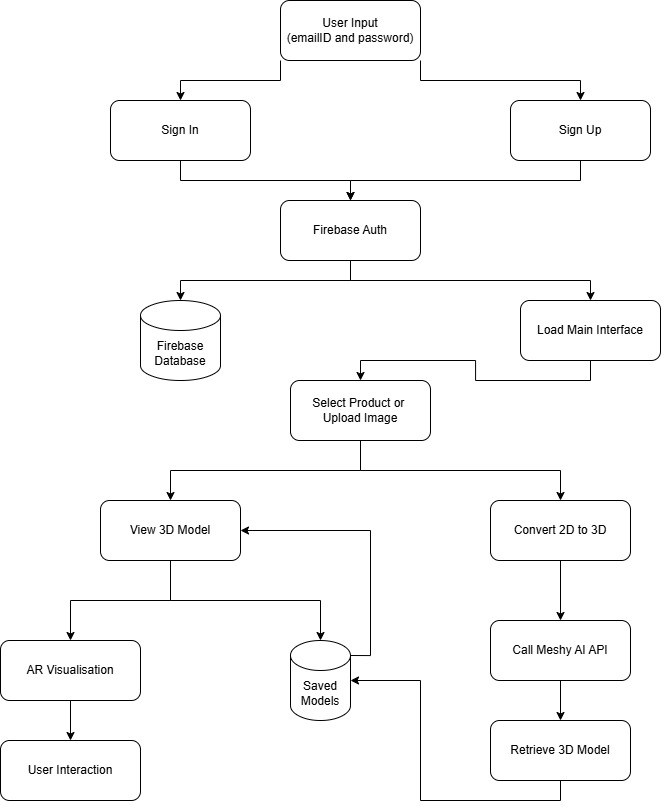
\includegraphics[width=0.9\columnwidth]{fig_p3_0}
\caption*{Figure 1}
\label{fig:1}
\end{figure}

\begin{figure}[H]
\centering
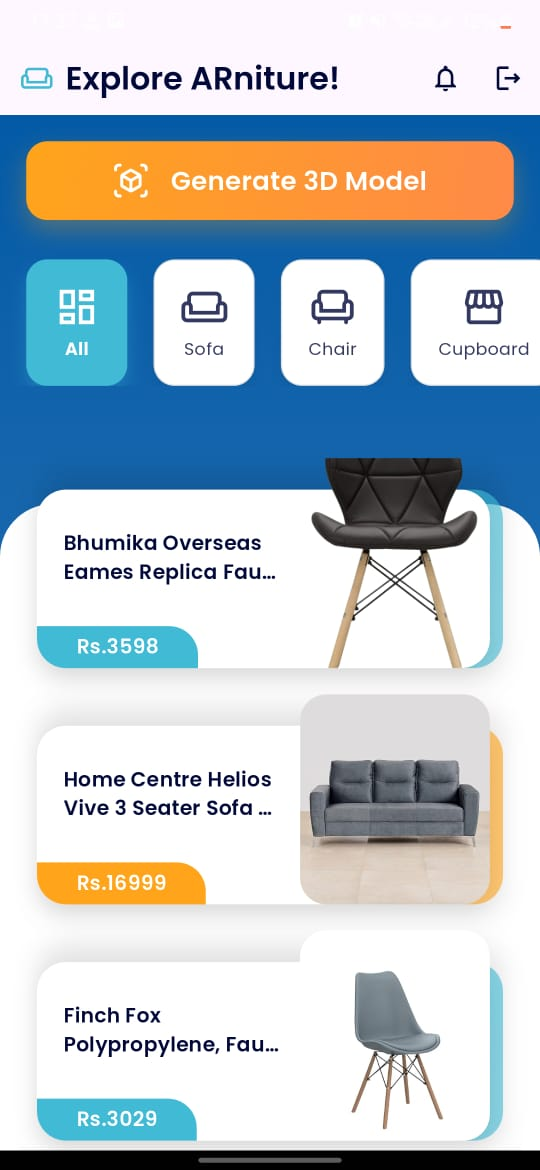
\includegraphics[width=0.9\columnwidth]{fig_p4_1}
\caption*{Figure 2}
\label{fig:2}
\end{figure}

\begin{figure}[H]
\centering
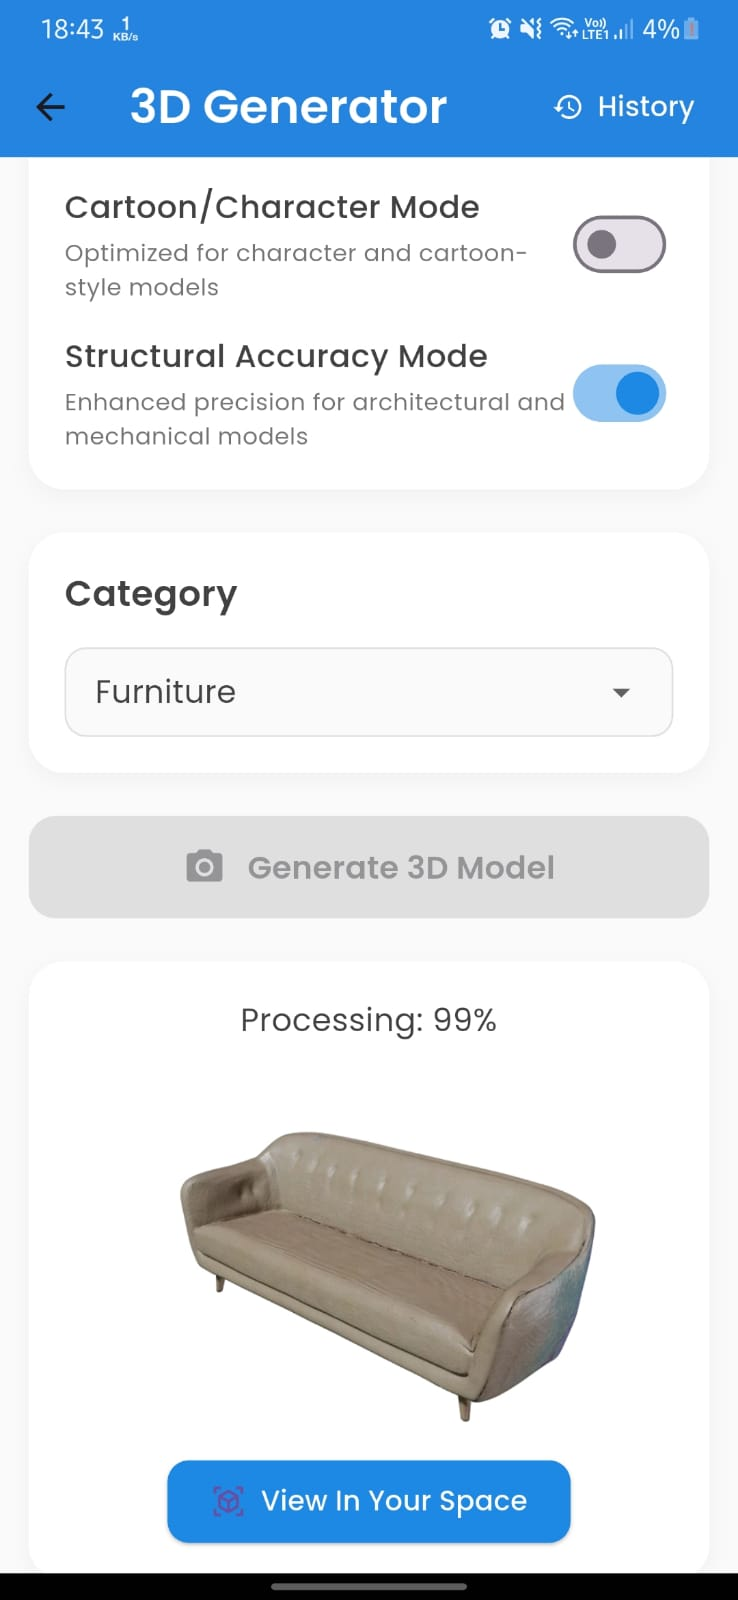
\includegraphics[width=0.9\columnwidth]{fig_p4_2}
\caption*{Figure 3}
\label{fig:3}
\end{figure}

\begin{figure}[H]
\centering

\includegraphics[width=0.9\columnwidth]{fig_p4_0}
\caption*{Figure 4}
\label{fig:4}
\end{figure}

\begin{figure}[H]
\centering
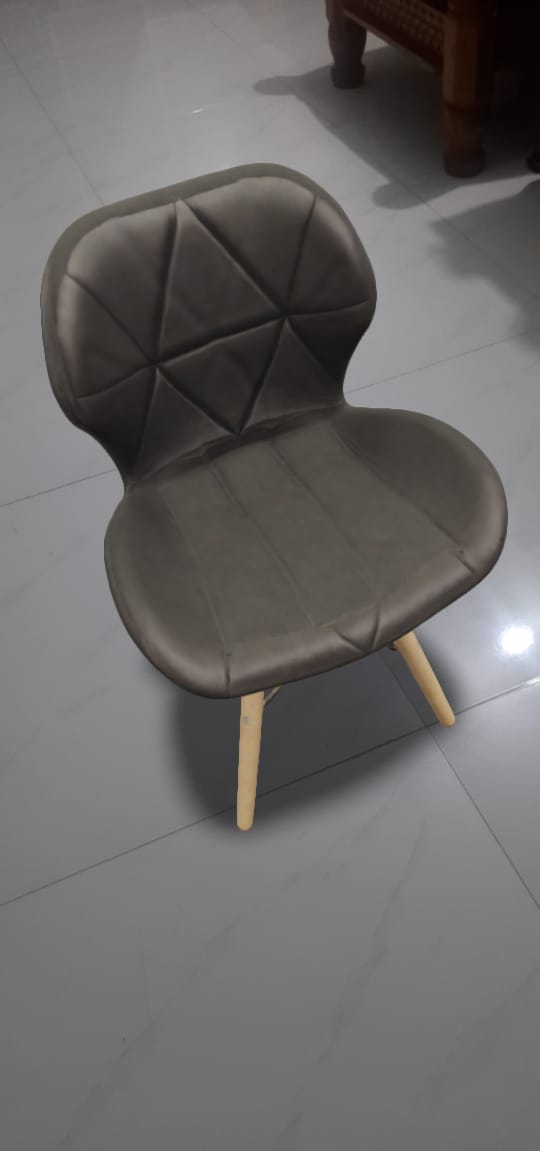
\includegraphics[width=0.9\columnwidth]{fig_p5_2}
\caption*{Figure 5}
\label{fig:5}
\end{figure}

\begin{figure}[H]
\centering
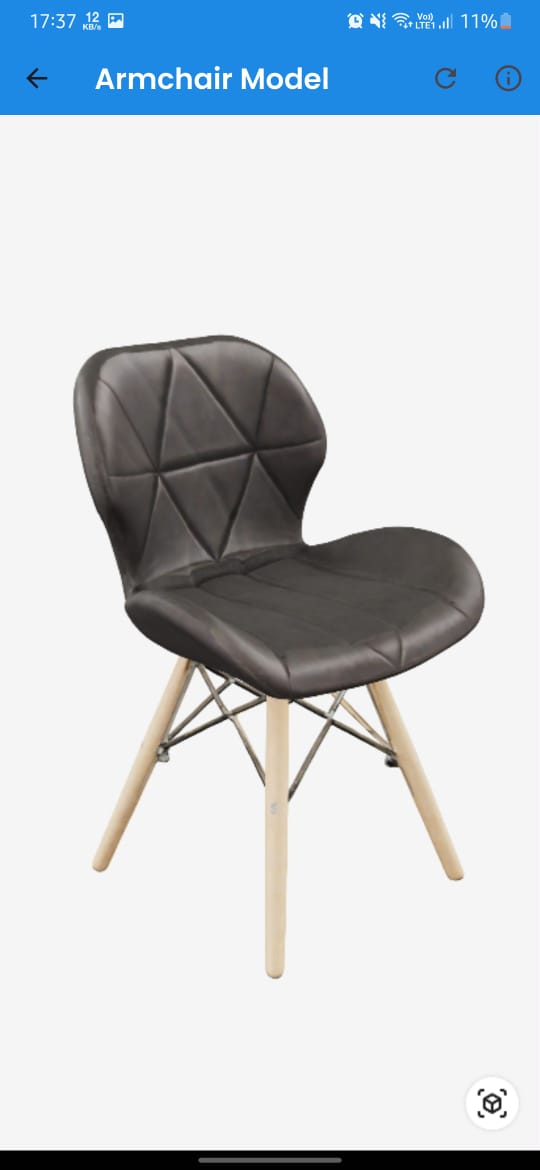
\includegraphics[width=0.9\columnwidth]{fig_p5_0}
\caption*{Figure 6}
\label{fig:6}
\end{figure}

\begin{figure}[H]
\centering
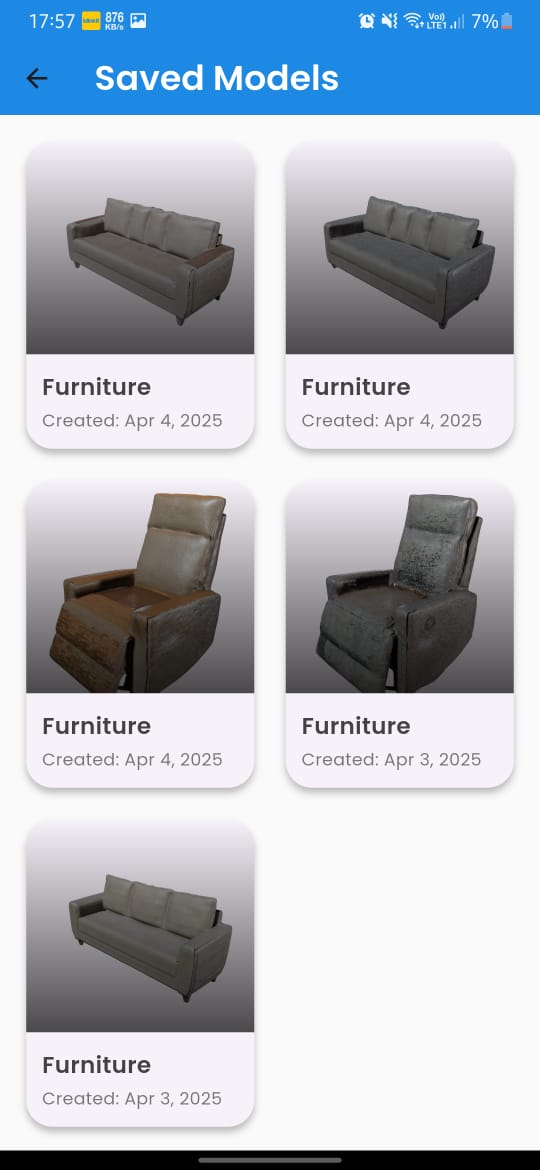
\includegraphics[width=0.9\columnwidth]{fig_p5_1}
\caption*{Figure 7}
\label{fig:7}
\end{figure}
\end{document}